\documentclass[journal]{IEEEtran}
% IEEE Transactions on Industrial Informatics -- anonymous regular-paper draft
% Compile: latexmk -pdf main.tex
\usepackage{amsmath,amssymb,amsfonts}
% Local XeTeX/Tectonic builds: route IEEEtran's ptm (Times) family requests to
% the legacy Times Type1 faces so metrics match the pdfLaTeX reference build;
% the latexmk -pdf (pdfLaTeX) path is unaffected.
\usepackage{iftex}
\ifxetex
  \DeclareFontFamily{TU}{ptm}{}
  \DeclareFontShape{TU}{ptm}{m}{n}{<->ptmr8t}{}
  \DeclareFontShape{TU}{ptm}{b}{n}{<->ptmb8t}{}
  \DeclareFontShape{TU}{ptm}{m}{it}{<->ptmri8t}{}
  \DeclareFontShape{TU}{ptm}{b}{it}{<->ptmbi8t}{}
  \DeclareFontShape{TU}{ptm}{m}{sl}{<->ptmro8t}{}
  \DeclareFontShape{TU}{ptm}{m}{sc}{<->ptmr8t}{}
\fi
\usepackage{graphicx}
\usepackage{booktabs}
\usepackage{tabularx}
\usepackage{array}
\usepackage[table]{xcolor}
\usepackage{stfloats}
\usepackage{placeins}
\usepackage{url}
\urlstyle{same}
% Cross-references and citations. The cite package renders IEEE-style citation
% groups ([14]--[16], [20], [21]) with hyperref support.
\usepackage{cite}
\usepackage[colorlinks=true,linkcolor=black,citecolor=black,urlcolor=black]{hyperref}
\hypersetup{bookmarksnumbered=true,
  pdftitle={AgentWorkShop: An Extensible Framework for Configurable Multi-Scenario Industrial Agent Integration},
  pdfauthor={Anonymous Authors},
  pdfsubject={IEEE Transactions on Industrial Informatics},
  pdfkeywords={industrial agents, industrial informatics, multi-agent systems, production system integration, process control, semantic data integration}}

% Float placement only; IEEEtran margins and body type remain unchanged.
\setcounter{topnumber}{4}
\setcounter{bottomnumber}{3}
\setcounter{totalnumber}{7}
\setcounter{dbltopnumber}{4}
\renewcommand{\topfraction}{0.95}
\renewcommand{\bottomfraction}{0.80}
\renewcommand{\textfraction}{0.03}
\renewcommand{\floatpagefraction}{0.72}
\renewcommand{\dbltopfraction}{0.95}
\renewcommand{\dblfloatpagefraction}{0.72}

% Tight but conventional float separation; body type and margins are unchanged.
\setlength{\textfloatsep}{8pt plus 2pt minus 3pt}
\setlength{\dbltextfloatsep}{8pt plus 2pt minus 3pt}
\setlength{\intextsep}{7pt plus 2pt minus 3pt}
\setlength{\abovecaptionskip}{3pt plus 1pt minus 1pt}
\setlength{\belowcaptionskip}{2pt plus 1pt minus 1pt}

% Evidence snapshot: integrated run 20260921184204-10lc.
% Artifacts: bench/results/20260921184204-10lc/{report.md,run.json,
% scenarios-benchmark.md,scenarios.json,metrics.csv,summary.json}.
% The agentteam-mission/agentteam-biax console logs and the two omp
% engine-turn transcripts were excluded from the archive by the repo's
% *.log ignore rule (see ARTIFACT-NOTES.md in that directory); their
% checked outcomes are recorded inside report.md and run.json.
% The four-arm ablation companion remains
% bench/results/20260921181234-e1lite/run.json.
\newcommand{\resEvidenceDate}{September~21, 2026, 19:08~UTC}
\newcommand{\resRun}{\texttt{20260921184204-10lc}}
\newcommand{\resCommit}{\texttt{e692df1}}
\newcommand{\resHarness}{\texttt{9f2756dce4a4cbb3}}
\newcommand{\resSeed}{42}
\newcommand{\resPhases}{20}
\newcommand{\resChecksTotal}{83}
\newcommand{\resChecksPass}{83}
\newcommand{\resChecksWarn}{0}
\newcommand{\resChecksFail}{0}
\newcommand{\resTotalWall}{26\,min}
\newcommand{\resDaqSamples}{55}
\newcommand{\resWriteP}{29.954\,ms}
\newcommand{\resTcpP}{47.8\,ms}
\newcommand{\resOpcP}{19.8\,ms}
\newcommand{\resMqttP}{19.3\,ms}
\newcommand{\resHttpP}{32.9\,ms}
% p95 per protocol line, same run: ~6 writes each. Recorded in the archive's
% metrics.csv (write_p95_ms) but reported in the body only since the 2026-10-12
% revision, so they live here rather than inline. Names must be letters only:
% \resTcpP95 would parse as \resTcpP followed by the characters "95".
\newcommand{\resTcpTail}{248.9\,ms}
\newcommand{\resOpcTail}{20.5\,ms}
\newcommand{\resMqttTail}{20.1\,ms}
\newcommand{\resHttpTail}{44.6\,ms}
\newcommand{\resWriteNperLine}{6}
\newcommand{\resAblationRun}{\texttt{20260921181234-e1lite}}
\newcommand{\resFullIntercept}{18/18}
\newcommand{\resNoInterlockIntercept}{12/18}
\newcommand{\resNoReadbackIntercept}{18/18}
\newcommand{\resUngatedIntercept}{12/18}
\newcommand{\resBackstop}{130.2\,s}
\newcommand{\resBackstopDrill}{134.7\,s}
\newcommand{\resPortFfive}{9/9}
\newcommand{\resPortCode}{0}
\newcommand{\resParamChecks}{4/4}
\newcommand{\resHitlLatency}{461\,ms}
\newcommand{\resMissionFrom}{200}
\newcommand{\resMissionTo}{204.704}
\newcommand{\resMissionPv}{204.70}
\newcommand{\resMissionTarget}{$204.704\pm0.75$}
\newcommand{\resBiaxSp}{30}
\newcommand{\resBiaxDaq}{19}
\newcommand{\resBiaxWrites}{3}
\newcommand{\resBiaxStart}{28.10}
\newcommand{\resBiaxFinal}{25.66}
\newcommand{\resBiaxTarget}{25.0}
\newcommand{\resBiaxTol}{0.7}
\newcommand{\resLlmWall}{156.3\,s}
\newcommand{\resGoalWall}{637.3\,s}
\newcommand{\resGoalFinal}{51.7}
\newcommand{\resJstar}{89.894}
\newcommand{\resJzero}{67.2}
\newcommand{\resControllerMin}{0.965}
\newcommand{\resControllerMean}{0.969}
\newcommand{\resControllerMax}{0.972}
\newcommand{\resInjStart}{31.25}
\newcommand{\resInjFinal}{32.17}
\newcommand{\resInjWrites}{2}
\newcommand{\resInjWall}{26.48\,s}
\newcommand{\resWwtpStart}{0.21}
\newcommand{\resWwtpFinal}{3.50}
\newcommand{\resWwtpWrites}{15}
\newcommand{\resWwtpWall}{169.27\,s}
\newcommand{\resWwtpCostStart}{181.5}
\newcommand{\resWwtpCostFinal}{179.1}
\newcommand{\resAnnealStart}{134.52}
\newcommand{\resAnnealFinal}{100.08}
\newcommand{\resAnnealWrites}{5}
\newcommand{\resAnnealWall}{102.76\,s}
\newcommand{\resAnnealSpeedFinal}{164}
\newcommand{\resAnnealSpeedTried}{176}
\newcommand{\resAnnealGain}{17.1\%}
% writeLockSeconds: node field default 30 s, constructor default 60 s; the
% online path enforces max(60 s, configured), so 60 s is the effective floor
% (unused in body since the pacing-window rewrite; kept for reference).
\newcommand{\resWriteLock}{60\,s}

% October 2026 deployment-scale campaign (v0.7.57), added with the revision.
% Artifacts: docs/benchmarks/benchmark-20261008045434/{report.md,benchmark.json,
% timeline.jsonl} (hardened pipeline; archived score 91/91 -- the 92/92 quoted
% in some audit notes belongs to same-day rerun benchmark-20261008135743);
% three consecutive full-suite runs benchmark-20261007194240|194413|194925
% (79/79 each, 237 total; an earlier 80-per-run tally counted one S7 report
% assertion that is not a logged check -- summarized in
% docs/benchmarks/EXPERIMENT-REPORT.md); regression suites
% scripts/testing/api-full-loop.mjs (53/53), tmp-e2e/hardening-ack-gate.mjs
% (34/34); docs consistency scripts/check-docs-sync.mjs (91/91).
\newcommand{\resPipeRun}{\texttt{benchmark-20261008045434}}
\newcommand{\resPipeTotal}{91}
\newcommand{\resPipeApi}{54}
\newcommand{\resCampaignRuns}{three consecutive}
\newcommand{\resCampaignTotal}{237}
\newcommand{\resCampaignApi}{45}
\newcommand{\resLoopTotal}{53}
\newcommand{\resAckTotal}{34}
\newcommand{\resDocsTotal}{91}
\newcommand{\resLinesLive}{34}
\newcommand{\resLinesRunning}{17}
\newcommand{\resChannelsLive}{112}
\newcommand{\resDaqOnline}{67}
\newcommand{\resWriteNodesLive}{77}
\newcommand{\resRecipesLive}{52}
\newcommand{\resBindingsLive}{385}
% approval->dispatch spans both campaigns: 8/9/9 ms (Oct 7-8), 9/6/6 ms (Oct 9).
\newcommand{\resHitlDispatchMs}{6--9\,ms}
\newcommand{\resLadderFrom}{66}
\newcommand{\resLadderTo}{63}
\newcommand{\resConsistencyErr}{0.0\,bar}
\newcommand{\resObsVerifyFast}{25.1\,s}
\newcommand{\resObsVerifyCadence}{245.2/245.1\,s}
\newcommand{\resCadenceWait}{218\,s}
\newcommand{\resWideRows}{869}
\newcommand{\resInspecRatio}{$100\%/100\%/99.9\%$}

% October 9, 2026 regression campaign (v0.7.57), same live instance.
% Artifacts: docs/benchmarks/benchmark-20261009021149 (extended, 92/92),
% benchmark-20261009024141 (90/90), benchmark-20261009033810 (90/90);
% timeline.jsonl per run (S4/S5 process records, HITL card events).
\newcommand{\resNovRuns}{\texttt{benchmark-20261009021149}/\texttt{-024141}/\texttt{-033810}}
\newcommand{\resNovTotal}{272}
\newcommand{\resNovApi}{54}
\newcommand{\resNovDeadband}{0.15\,g}
\newcommand{\resNovZigzagFrom}{64}
\newcommand{\resNovZigzagTo}{63}
\newcommand{\resNovCorrFrom}{63}
\newcommand{\resNovCorrTo}{65}
\newcommand{\resNovWeights}{$32.49/32.33/32.22$\,g}
\newcommand{\resNovCadenceReject}{69\,s}
\newcommand{\resNovCardId}{\texttt{ap-2950a5b6}}
\newcommand{\resNovRunId}{\texttt{rr-51b0a0ac}}
\newcommand{\resNovScheme}{hold-pressure micro-up (sensitivity excitation step)}
\newcommand{\resNovSlope}{0.052\,g/bar}
% Oct 9 diagnostics: three-run distribution, not the single worst run.
% runs 021149/024141/033810: rows 663/843/861, in-spec 100.0/96.4/94.0%,
% std 0.042/0.186/0.237 g. \resNovInspec/\resNovWideRows/\resNovStd below are
% the single third-run values, superseded by the range macros in the body.
\newcommand{\resNovInspecRange}{94.0--100.0\%}
\newcommand{\resNovStdRange}{0.04--0.24\,g}
\newcommand{\resRowsRange}{663--869}
\newcommand{\resNovInspec}{94.0\%}
\newcommand{\resNovWideRows}{861}
\newcommand{\resNovStd}{0.24\,g}


\newcommand{\system}{the platform}

\begin{document}
\bstctlcite{IEEEbstctl}

\title{AgentWorkShop: An Extensible Framework for Configurable Multi-Scenario Industrial Agent Integration}

\author{Anonymous Authors}
\markboth{IEEE Transactions on Industrial Informatics, Submitted Manuscript}{AgentWorkShop Industrial Agent Integration}

\maketitle

\begin{abstract}
Industrial agent applications must connect collaborative reasoning,
production context, and heterogeneous plant interfaces while preserving a
traceable path from a task proposal to its process outcome. This paper
presents AgentWorkShop, an extensible framework for configuring these
capabilities across industrial scenarios. Its architecture combines team
and task orchestration with replaceable strategy adapters; analysis,
retrieval, dataset, and model services; line--product--recipe--run context;
semantic acquisition and write-control nodes; and typed interfaces for
onboarding and extension. Scenario-specific signal maps, protocol bindings,
objectives, and guards configure process integrations while shared
collaboration and operational services remain reusable. Candidate actions
enter either bounded node exploration or an operational recipe workflow,
where dispatch evidence, process observations, and retained versions follow
route-specific lifecycles. Evaluation exercised acquisition over five protocol families, controlled
writes over four routes, strategy and controller substitutions, and four
simulator process configurations. Each process had one seed-42 trajectory;
all reached their declared terminal targets, two near a boundary. Nine
sequential deployment-suite executions recorded 782 deterministic
assertions.
A single accelerated injection-molding trajectory linked four pressure trials
from 45 to 65 bar, each approved by the scripted test harness, to a measured weight
change from 31.28 to 32.30 g and subsequent recipe retention.
The evidence supports
configuration-based reuse across the exercised scenes and interfaces; all
process results are simulator-based, and later checks exposed
current-interface cadence limits. It does not establish physical transfer,
broad plant coverage, or comparative optimization benefit.
\end{abstract}

\begin{IEEEkeywords}
Industrial agents, industrial informatics, multi-agent systems, production
system integration, process control, semantic data integration.
\end{IEEEkeywords}

\IEEEpeerreviewmaketitle

\section{Introduction}
\IEEEPARstart{L}{arge} language model (LLM) agents are moving from advising
industrial operations to acting on them: recent systems generate control
updates for industrial cyber-physical systems from multi-modal input
\cite{huang2026made}, pair each factory module with an LLM agent that
dispatches skills over a tool protocol \cite{koehle2026llmdriven}, allocate
work among cooperating agents \cite{lim2025llmenabled,zhao2026shopfloor},
and have been studied as real-time controllers of a robot production line
\cite{waseem2026pretrained}. What these demonstrations leave implicit is
everything that surrounds the proposal: who may change which parameter, which
limits are active for the current product and recipe, whether a human
approved, whether the device accepted the command, and whether the process
improved.

Because these concerns are normally embedded in application code, they are
rebuilt per process, protocol, and agent framework---duplicated drivers,
ad-hoc permission checks, logs untied to decisions. The four scenario plants (simulated in this paper) differ---injection molding, wastewater treatment (WWTP), annealing,
and BOPET (biaxially oriented polyethylene terephthalate)
film---but all need an auditable bridge from a
team-level task to heterogeneous acquisition and control nodes. Industrial
LLM work to date has largely targeted generation, diagnosis, and
single-domain control \cite{liu2026agents4plc,jiang2026agentic}.

\looseness=-1 \system{} addresses this execution gap through member--node bindings (a
member being an engine-backed channel identity) and shared line, product,
recipe, and run context. The response is
organizational rather than algorithmic: each intervention leaves a
separate evidence record per governed stage, from admission through
compensation (Section~\ref{sec:mech}). Nodes expose engineering quantities
rather than register addresses, and one governed member--node binding path
serves every client.

The paper makes four contributions:
\begin{enumerate}
\item a \textbf{capability-based industrial execution architecture} connecting
agent-team identity, semantic data-acquisition (DAQ) and write-control (DCW,
the platform's node-class tag)
nodes, heterogeneous protocol drivers, and line--product--recipe--run context,
with task membership distinct from physical-write authority and a
default-manual line master switch;
\item a \textbf{reusable integration boundary} of self-describing node and
driver contracts across six protocol families (five instantiated as lines,
four exercised for governed writes), versioned production objects, plugin
extension points, and a typed software development kit (SDK), into which an
onboarding contract projects scenario blueprints while process models and
policies stay external;
\item an \textbf{evidence-preserving governed intervention workflow}
separating admission, optional approval, actuation, three-level write
acknowledgment with post-write verification, verdict, compensation, and
backstop---the grading rule stated falsifiably; and
\item a \textbf{layered evaluation} exercising one governed path through
protocol closure with mechanism ablation, agent-team missions, a
deterministic controller loop, concurrent process missions, and a
deployment-scale regression campaign on a multi-line instance
(Section~\ref{sec:eval}).
\end{enumerate}
Scope, revisited in Section~\ref{sec:limits}: real protocol stacks execute
against author-implemented simulators; fast regulation,
certified protection, physical-plant transfer, and optimizer ranking are
outside the claims. The governed path is proposer-agnostic---prompt content
is never authority and admission re-resolves per request---so the scripted
proposers of Section~\ref{sec:eval} exercise the same contract an
engine-issued proposal would face.

\section{Related Work}
\label{sec:related}
\subsection{LLM Agents in Industrial Control: From Generation to Governance}
\looseness=-1 Agent-based manufacturing and supervision have long linked
organizational roles to plant
capabilities \cite{leitao2009agentbased,biskupovic2025supervision}, and
LLM-oriented industrial work now spans PLC generation and verification
\cite{liu2026agents4plc} and direct plant-facing action---context-aware
control \cite{wu2025instructmpc}, digital-twin fault handling
\cite{gill2025llmdt}, and natural-language machine
control over OPC UA \cite{hofmann2025nlc}---without production-scoped
admission, per-request re-checking, or graded write evidence.
\looseness=-1 The closest systems (Table~\ref{tab:nearest}, as reported in
their publications) target the control action itself---multi-modal
control-update generation behind a safety layer \cite{huang2026made},
module-scoped skill dispatch over a six-module plant
\cite{koehle2026llmdriven}, and pretrained LLMs \emph{inside} the control
loop as real-time controllers \cite{waseem2026pretrained}, a layer below
\system{} so the roles are complementary---while agent-allocation work
\cite{lim2025llmenabled,zhao2026shopfloor} distributes tasks, not governed
writes. A recent review frames agentic AI's industrial value as
safety-aware human-in-the-loop (HITL) decision support rather than autonomous
control authority \cite{jiang2026agentic}---the mechanism set here makes
that concrete.

\begin{table*}[!t]
\centering
\caption{Closest LLM-based industrial control systems versus \system{}
(venue, LLM role, write path, production-scoped authority, write evidence).}
\label{tab:nearest}
\scriptsize
\setlength{\tabcolsep}{3.4pt}
\renewcommand{\arraystretch}{1.0}
\begin{tabular}{@{}>{\raggedright\arraybackslash}p{2.55cm}>{\raggedright\arraybackslash}p{3.1cm}>{\raggedright\arraybackslash}p{3.3cm}>{\raggedright\arraybackslash}p{3.9cm}>{\raggedright\arraybackslash}p{3.9cm}@{}}
\toprule
System (venue) & Role of the LLM & Plant write path & Authority \& production context & Write evidence \& verification \\
\midrule
MADE, ICCAD~2026 \cite{huang2026made} & multi-modal control-update generation & generated commands + safety layer & HITL verification of outputs; task-level checks & task success over scripted evaluations \\
K{\"o}hle et al., ETFA~2026 \cite{koehle2026llmdriven} & per-module agents, MCP skill dispatch & skill invocation via OPC UA/MQTT & module-scoped skills & task-resolution rate (6-module plant) \\
Lim \& Kovalenko, CASE~2025 \cite{lim2025llmenabled} & capability exploration across agents & architecture-level & resource-matching scope & architecture evaluation \\
Zhao et al., AEI~2026 \cite{zhao2026shopfloor} & shop-floor task dispatch & workshop experiments & coordination layer & dispatch/execution performance \\
Waseem et al., Mach.\ Learn.\ Eng.\ 2026 \cite{waseem2026pretrained} & real-time controller in the loop & direct loop actuation (robot line) & prompt-level constraints & line KPIs under LLM control \\
\midrule
\rowcolor{gray!12}
\textbf{\system{}} & \textbf{replaceable strategy slot} & \textbf{governed write path: admission, HITL, dispatch, readback} & \textbf{member--node bindings; line master switch; product/recipe-scoped limits} & \textbf{graded acknowledgment; harness-checked three-way consistency; attributed journal; compensation; backstop} \\
\bottomrule
\end{tabular}
\end{table*}

\subsection{Frameworks, Standards, Run-Time Guarantees, and Automation Practice}
\looseness=-1 The Model Context
Protocol (MCP) standardizes multi-agent tool interfaces \cite{mcp2024};
its tools carry advisory annotations but no production
context---line, product, or recipe---and no record separating admission
from execution. ISA-88 and ISA-95 model recipes and operations
\cite{isa88,isa95}, and \system{}'s versioned recipes instantiate
a reduced subset of that stack; the governed
life cycle transposes run-to-run (R2R) control disciplines \cite{moyne2000r2r}
onto a supervisory write path.
A separate line enforces run-time guarantees on LLM agents---guard agents
\cite{xiang2024guardagent}, schema-level behavioral constraints
(AgentSpec \cite{wang2025agentspec}), and capability-based
information-flow control (CaMeL \cite{debenedetti2025camel}), the closest
software-agent analogue of the rule that prompt content is never authority;
they gate software tool calls and data flow, not plant writes; their
policies could compile onto this substrate.

\looseness=-1 Permissions, range checks, approvals, and audit trails long existed in
distributed-control-system (DCS) and SCADA practice---versioned batch
recipes and electronic batch journals under 21~CFR Part~11 and GAMP~5
\cite{part11,gamp5}, second-channel monitoring and advisory
operations in NAMUR open architecture
\cite{namur2017noa}, and setpoint adaptation in run-to-run control---while
IEC~62443 codifies their security counterpart \cite{iec62443-3-3} and
formal shielding, control-barrier functions, and simplex run-time assurance
offer stronger properties
\cite{alshiekh2018shielding,ames2017cbf,sha2001simplex}. Graded command
confirmation itself has telecontrol ancestry: DNP3's select-before-operate
exchange \cite{ieee1815dnp3} and IEC~60870-5's command-acknowledgment cycle
\cite{iec60870104} confirm a command at the protocol and application layer;
\system{} grades above them, against production context and actor
attribution. Against that
practice the difference is the proposer: a machine-generated agent identity
rather than a presupposed human operator, so admission binds to member
authority, prompt content stays inert, and intervals are re-evaluated per
request against live product and recipe state. No safeguard above is claimed
as an invention---what is new is their composition into this one
proposer-agnostic path, whose evidence
states---graded acknowledgment, verdict, compensation---survive strategy
replacement; the three-way check is a supervised special case of
classical data reconciliation
\cite{crowe1996reconciliation}.
\system{} implements source-dependent checks and a rule-based backstop
(Section~\ref{sec:agentloop}), no formal protection guarantee; human
oversight likewise requires more than an approval dialog
\cite{bainbridge1983ironies}.

\section{System Architecture}
\label{sec:arch}
\looseness=-1 \system{} fills this slot: it links team coordination to plant interaction through industrial nodes
and production context (Fig.~\ref{fig:arch}). Five planes separate the
concerns: a \emph{team} plane owns member identity, task state, and a
member-written episodic memory retrieved by hybrid search; an
\emph{integration} plane owns protocol acceptance, readback, freshness, and
transport errors, presenting devices as semantic nodes whose stream feeds both
the agent and a live plant-mirror view; a \emph{governance} plane owns
admission, approval, actuation, acknowledgment grading, three-way consistency,
verdict, compensation, and rollback; an \emph{operations} plane attaches line,
product, recipe, and run context while PLC protection stays independent; and
an \emph{extensibility} plane admits plugins, drivers, agent tools, panels,
and SDK clients through sanctioned registration services. Scenario knowledge
sits in blueprints, signal maps, predicates, and driver configuration---not
in team scheduler, approval service, or persistence code; members are interchangeable
across 14 engine adapters under preserved identity, and 118 declared
settings (40 hot-reloadable, the rest restart-scoped) plus the typed SDK make
team topology, bindings, and limits data rather than code. In every plane the
execution path is unchanged---a scenario supplies data
and strategy (Fig.~\ref{fig:arch}).

\begin{figure*}[!t]
\centering
% 0.88\textwidth with source fonts sized so the printed text stays >=6pt;
% narrower includes drop the card body below the legibility floor
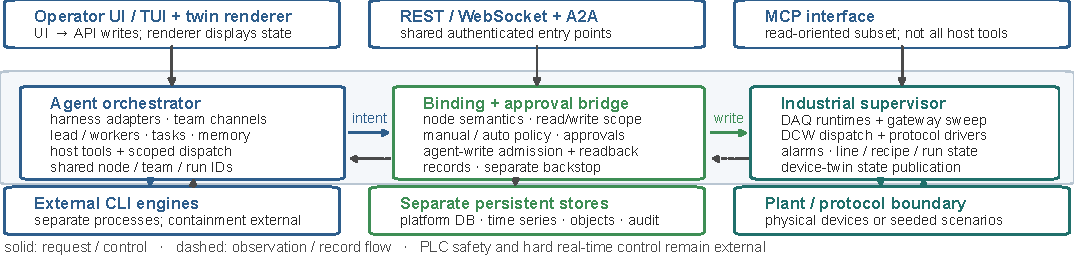
\includegraphics[width=0.88\textwidth]{resources/fig2-architecture.pdf}
\caption{System architecture and execution boundaries: platform services
around shared stores, operator interfaces above, and agent engines, data
stores, protocol endpoints, and the plant kept separate. Shared identifiers provide
attribution but do not make storage and actuation transactional.}
\label{fig:arch}\end{figure*}

\subsection{Supervisory Core and Nodes}
\looseness=-1 The Node.js core hosts channel routing, industrial services, and protocol
adapters. A channel contains a lead, workers, tasks, messages, and retrievable
memory, deployed through WebSocket, MCP, A2A, REST, CLI, or TUI entry points;
channel membership alone confers no write authority.

DAQ nodes convert device readings to engineering quantities across four
modalities---scalars, vector profiles, image frames carrying content
fingerprints, and mirrored manufacturing-execution-system (MES)
records---so plant data-shape heterogeneity does not reach the team loop. MES endpoints are reached in two
interchangeable modes---\emph{mirror}, pulling MES records through the same
acquisition pipeline as any field device, and \emph{direct}, declaring read
and write mappings against the MES interface. DCW
nodes translate engineering setpoints into driver commands and, where
supported, readback; per-node runtimes manage timing, and gateway services supply
connection state, recipe context, and write bookkeeping. The acquisition
surface declares six protocol families, five with drivers today---Modbus TCP,
Modbus RTU-over-TCP, OPC UA, MQTT, HTTP/REST, and an S7
stub that fails loudly until its driver lands; the write surface is six
drivers over the five writable families plus MES REST, with the evaluation's
mock driver registered explicitly and outside that count; the evaluation
instantiates five families as lines (Section~\ref{sec:protocol}).
The deployment reaches author-implemented dynamic simulators through the same
node and driver contracts a plant would use; they are deterministic per seed,
not validated digital twins. The first reuse boundary is declarative---signals,
units, scaling, precision, and driver configuration---and the team loop is
unchanged; fast regulation and independent protection stay in plant
controllers.

Driver contracts are deliberately narrow: a driver declares how a semantic
quantity maps to its transport payload, whether the endpoint is writable, and
whether a readback is available, while the controller resolves member authority
and active limits. Errors attach to the
request rather than one success flag, and register addresses and byte order
appear only here, so a new fieldbus family leaves the loop untouched. Undeclared drivers fail loudly: a node whose driver is not registered is
rejected at creation and connection test rather than silently served by a
mock (Section~\ref{sec:hardening}).
Acquisition is supervisory rather than hard real-time: each DAQ node runs its
own cadence under a rotating sweep, so a slow endpoint delays only its own
samples, and the verdict stage queries the timestamped, quality-stamped
history rather than issuing a blocking read.

\subsection{Bindings, Context, and Reuse Boundaries}
\label{sec:reuse}
A member--node binding grants access to a sanctioned tool on a specific node and
selects automatic or approval-mediated execution. Line permissions (none,
read-only, operate) authorize binding creation and mutation; runtime
invocation is authorized by the persisted capability, not channel membership.
Intervals are re-checked every request instead of cached, so revoking
a binding or switching the recipe takes effect on the next request; the same path
serves a console, a harness, and an agent engine, because authority does not
depend on the client---only the evidence record differs.

Production objects are versioned rather than overwritten: a recipe is dispatched
against a known-good version, reverted non-destructively, and compared with the
values actually applied, and an intervention is read against the definition
that was active when it was admitted. Plugins register hooks, routes, agent tools, drivers,
and panels only through sanctioned services, so an added driver inherits
admission, readback, and evidence capture. Scenario reuse is bounded by an onboarding contract: the engineer declares a
blueprint (devices, signals, units, roles, setpoints); a differential
``ensure'' pass creates missing devices, repairs drift, verifies
connectivity, and projects it into semantic nodes and a recipe; a channel is
built from the team template, and a mission supplies objective, guards,
response windows, and policy. A
BOPET worker proposes casting-speed, fast-roll, or rail-width changes through
bound DCW nodes; the other three scenarios reuse the same pattern
(Section~\ref{sec:scenarios}). The stores share identifiers, not a
transaction domain: a device may accept a write even if bookkeeping fails.

\subsection{Governed Optimization Task Life Cycle}
\label{sec:tasklifecycle}
A governed optimization task is a life cycle rather than a single tool call, and
\system{} exposes each transition separately. The task enters a channel carrying
goal, line, product, recipe, run, and task identifiers; a lead member claims it
and hands it to a worker holding member--node bindings on the relevant nodes,
whose fixed job then repeats: read the controlled quantity over a
bounded window, propose a setpoint inside the resolved interval, invoke the
governed write, wait for the response, and record a verdict
(Section~\ref{sec:procedure} instruments it).

Each iteration leaves more than a written value: the write opens an
optimization record carrying prior and requested values, the admitting
interval, the acting member, and timestamps; the acknowledgment grade and,
where supported, the readback close the command path; the journal attributes
the change; and attainment is computed against the scenario predicate while
the task closes with a workflow terminal state (per-intervention detail in
Section~\ref{sec:mech}). This bounds what ``automatic optimization''
means here: a
controller, a scripted policy, a conventional optimizer, or an agent engine may
occupy the strategy slot, while authority, evidence, and closure stay on the
platform.

\begin{figure}[!t]
\centering
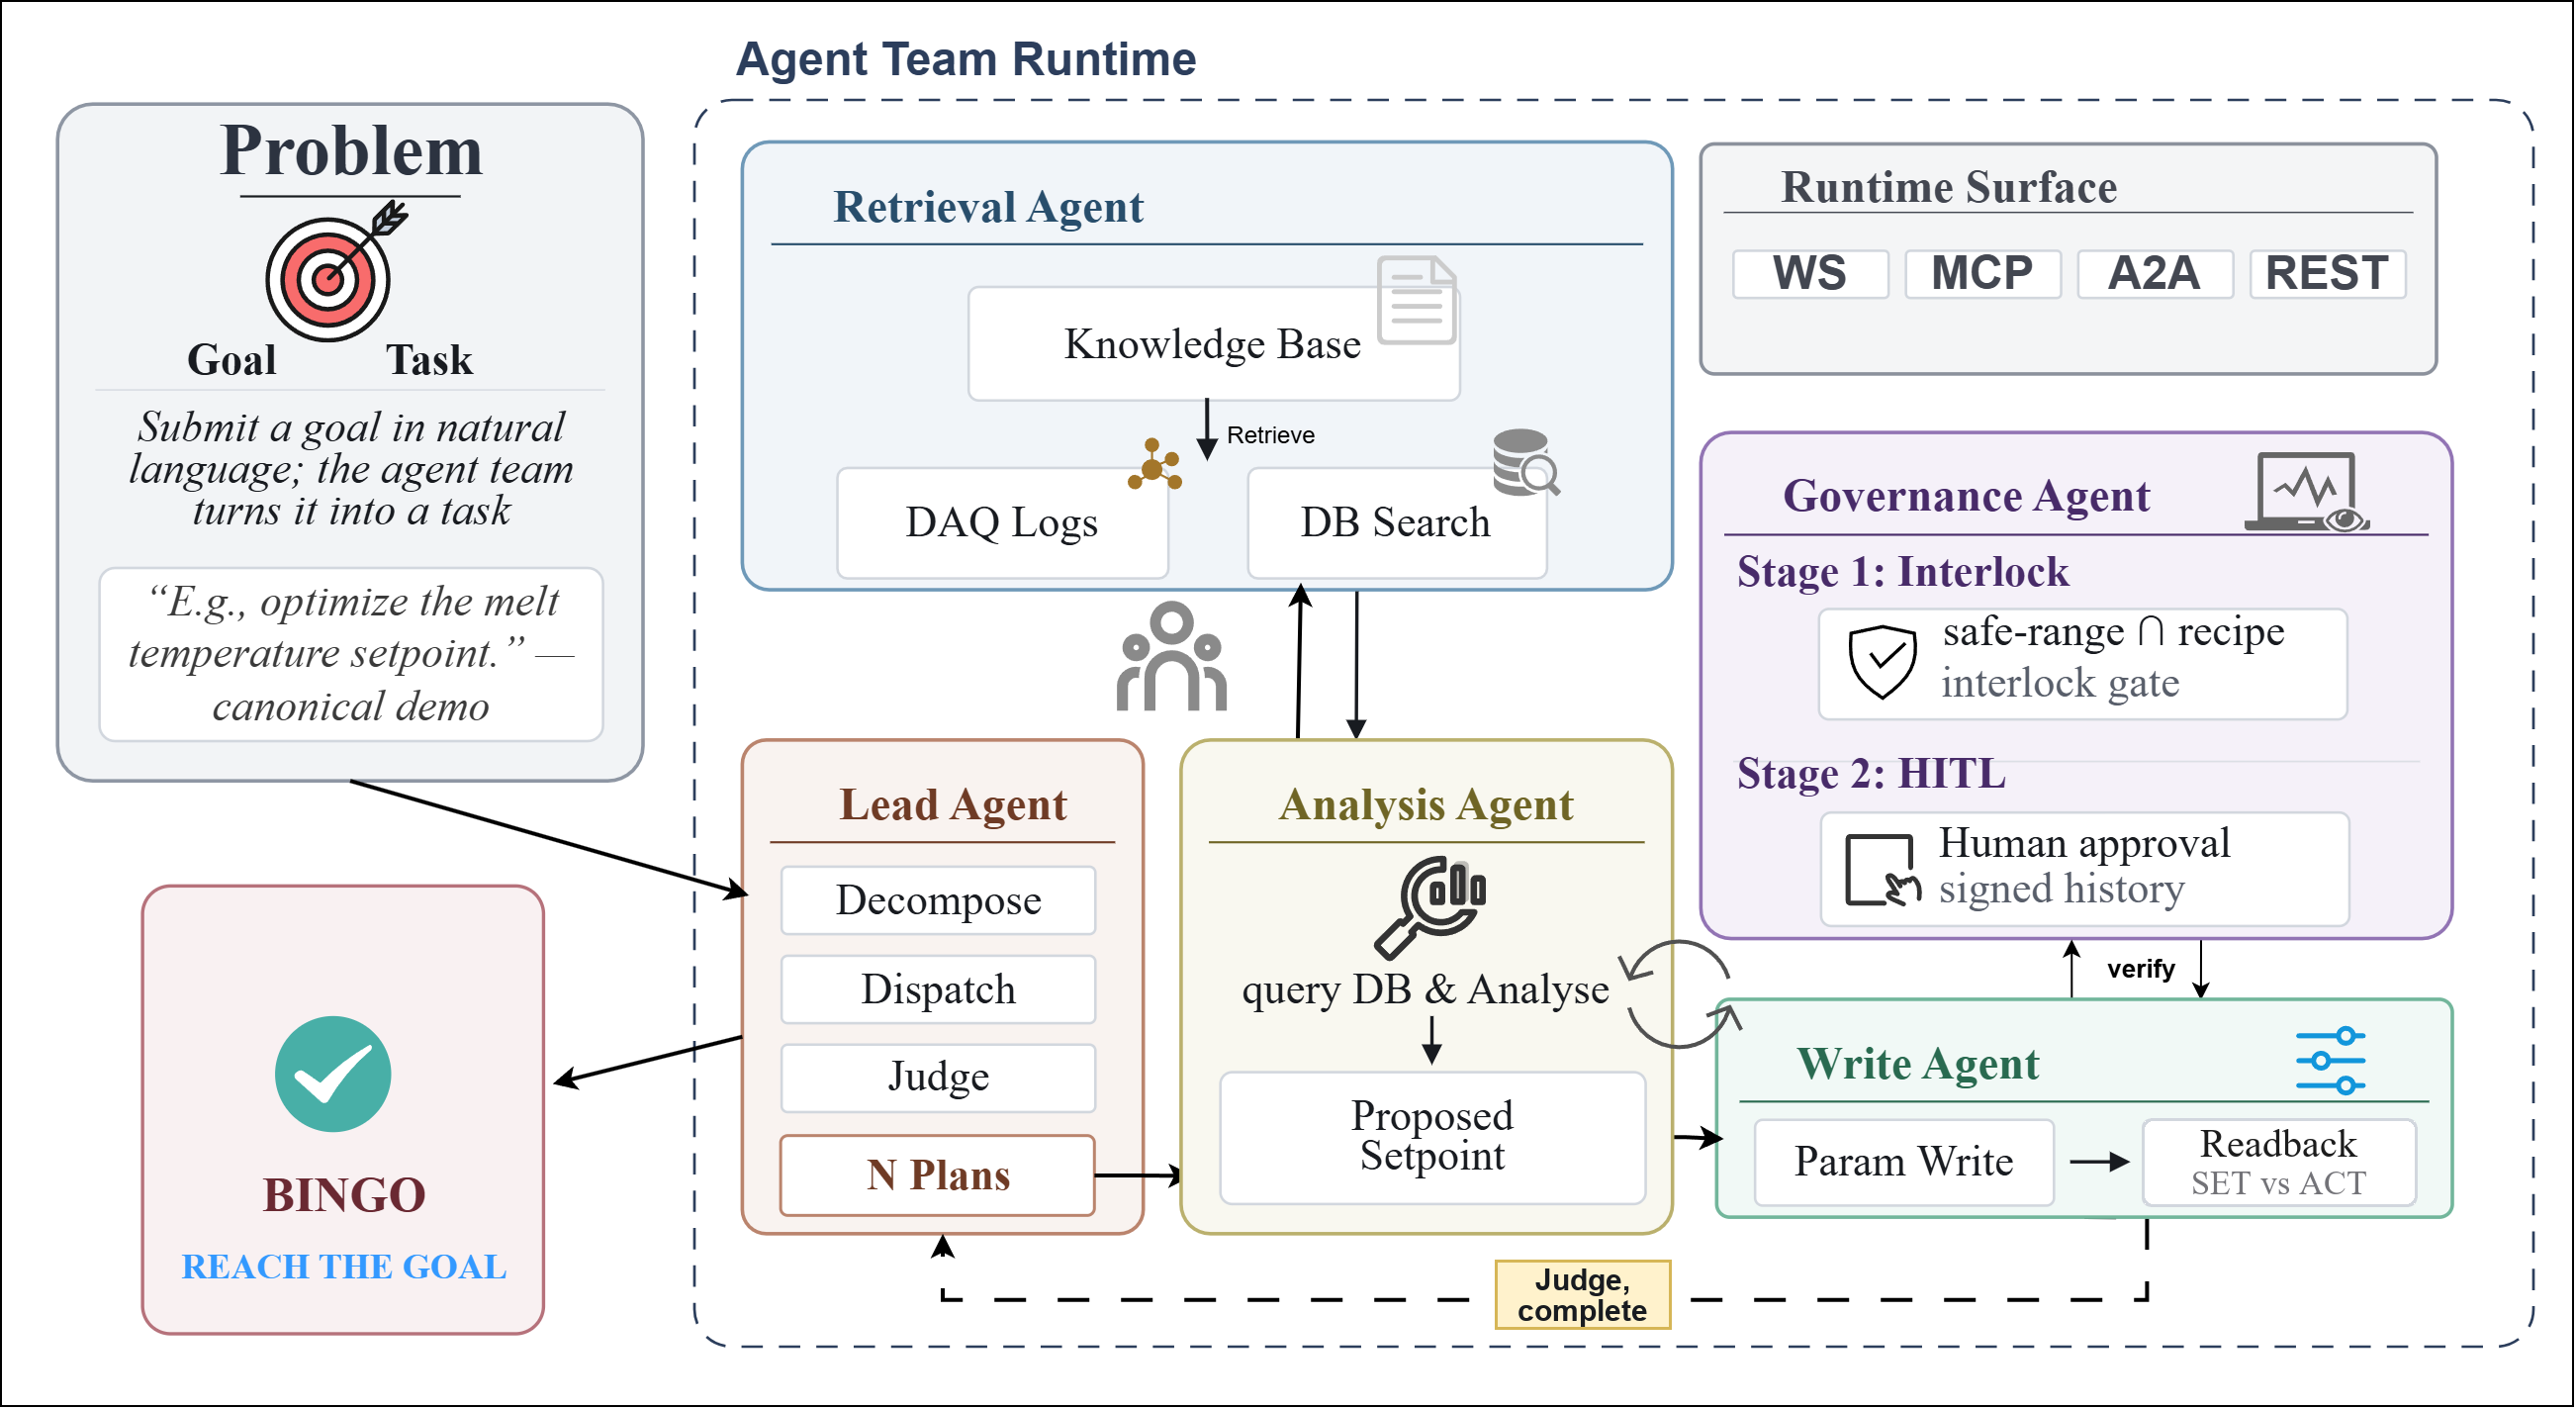
\includegraphics[width=\columnwidth]{resources/aws_fig3-flat.png}
\caption{Implemented agent-team runtime. A natural-language goal enters as
a task; the lead agent decomposes and dispatches plans; retrieval and
analysis produce the proposed setpoint (the LLM engine occupying a
replaceable strategy slot). The governance stages are deterministic platform
logic: Gate~1 applies the Eq.~\eqref{eq:admission} interlock, Gate~2 the
approval wait; the write agent reads back the value actually present (SET
versus observed ACT), and the judge records keep, rollback, or uncertain;
every step is journaled with actor attribution. The block labeled
``Governance Agent'' denotes these deterministic platform stages, not a
model-bearing agent; the judge annotation is the caller's verdict-tool
invocation.}
\label{fig:runtime}
\end{figure}

\section{Governed Execution Mechanisms}
\label{sec:mech}
A supervisory intervention must preserve distinctions that an agent tool call
usually collapses---permission to propose, admission of a value, driver
acceptance, device confirmation, process response, a caller's verdict, and
compensation---and \system{} exposes these as separate evidence states.
Three design commitments generate that separation: model output is treated
as an untrusted proposal, never as authority; evidence is graded by what is
observed rather than by what was claimed; and failure states are surfaced
for inspection rather than absorbed into a success flag.
Fig.~\ref{fig:runtime} shows the implemented agent-team
runtime that carries these steps; the governance and write stages drawn in
the figure are deterministic platform logic---no model output can admit,
approve, or confirm a write (Gates~1--2 of Fig.~\ref{fig:runtime}). A governed intervention is
one transaction in the audit-trail sense: every step
leaves its own evidence record, while execution and recovery are deliberately
not atomic with device state (Section~\ref{sec:limits}).
Six invariants organize the path---binding-resolved authority (never channel
membership or prompt content), Eq.~\eqref{eq:admission} admission,
fail-closed approval waits on manual bindings, graded rather than
success-flag acknowledgment, checkable three-way consistency, and
separately admitted compensation---each specified in the subsections that
follow, and every agent-originated path to the plant passes through the
same governed write.

\begin{figure}[!t]
\centering
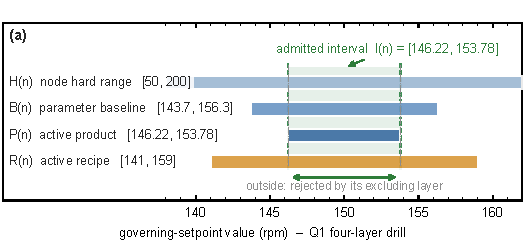
\includegraphics[width=\columnwidth]{resources/fig-admission.pdf}
\vspace{1pt}
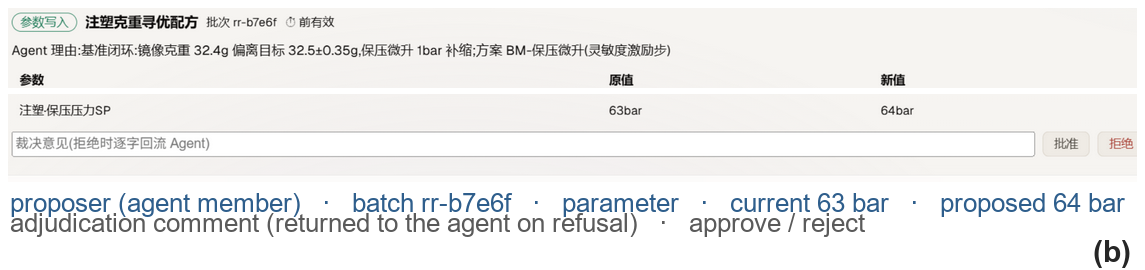
\includegraphics[width=0.78\columnwidth]{resources/hitl-card-crop.png}
\caption{The admission boundary and its human-approval gate, on the running
benchmark line. (a)~The Eq.~\eqref{eq:admission} interval geometry: four declared,
versioned bounds narrow to the admitted interval; a proposal
outside it is rejected by its excluding layer (the Q1 four-layer drill).
(b)~The structured approval card on a manual binding (live system, gloss
added): machine-checkable fields are separated from the proposer's
display-only reasoning; the comment returns to the member on refusal
(Section~\ref{sec:hitl}).}
\label{fig:hitl}
\end{figure}

\subsection{Task, Observation, and Admission}
\label{sec:objective}
The strategy receives a task and goal in production context and decides what
to propose and when to stop; the platform governs execution over semantic node
parameters---pressure, dosing rate, line speed, rail
width---in engineering units.

\looseness=-1 For an ordinary agent setpoint request on node $n$, the
admission interval is
\begin{equation}
\mathcal{I}_n(t)=\mathcal{H}_n\cap\mathcal{B}_n
                 \cap\mathcal{P}_n(t)\cap\mathcal{R}_n(t),
\label{eq:admission}
\end{equation}
where $\mathcal{H}_n$ is the mandatory hard engineering range (finite and
non-empty at node creation) and the remaining terms the baseline,
active-product, and active-recipe limits; a missing optional limit
contributes no restriction, so the interval is always defined, and $t$ is the
admission instant, re-resolved at execution. Should a configuration empty the
intersection, every write is rejected with the excluding layer named, so the
misconfiguration surfaces at the first write. The interval form is
deliberate: every bound is a declared, versioned object that an audit can
replay against the active product and recipe, and rejection is decidable and layer-attributable, where a learned
feasibility model offers neither
(Fig.~\ref{fig:hitl}a)---a decidability claim, not a safety certificate.
It bounds one parameter at a time---joint,
cross-variable windows live in scenario guards---and bounds magnitude, not
intent: availability, binding state, and approval policy are checked
separately, and in-window but adverse sequences surface at verdict and
compensation (Section~\ref{sec:scenarios} reports two).

\subsection{Semantic Write, Pacing, and Source-Specific Routes}
\label{sec:nodeexec}
A semantic card exposes quantity, unit, precision, range, value, freshness,
and recipe context; the controller resolves binding and limits, the driver
serializes the command, and the acknowledgment grade closes the
command path, never the process-response path (Section~\ref{sec:ack}). Two write-spacing windows pace governed loops, never
the plant: online writes---agent- or human-origin---sit at least 60\,s apart
with a hold window after success (HTTP~429 inside it); a per-recipe dispatch
interval anchored at the \emph{approval} instant is restart-persistent, so
alternating identities cannot reset it; and a 300\,s per-line trial cadence
damps same-line trials from any origin. Recipe-dispatch and rollback writes
are exempt. \texttt{AW\_BENCH\_MODE=1} admits harness-declared arms that
relax the soft window or readback---never the hard range.

\looseness=-1 Four governed routes---agent tools, human-origin writes, recipe
dispatch, and rollback compensation---reach the same driver through one
admission and journaling entry point, the hard range included; recipe
dispatch adds run context---the line-scoped execution window, the reduced
ISA-88 batch/lot notion---validated at save time. Hold heartbeats (periodic
re-dispatch of the stored setpoint) are the one non-governed re-dispatch:
off by default, stopped by line stop or driver change, and re-applying the
stored value without re-admission---plant-facing state maintenance, not an
agent path. Line start installs active context before recipe parameters
dispatch individually, and line stop clears it; these multi-step operations
are not atomic with device state.

\subsection{Write Acknowledgment as Three-Level Evidence}
\label{sec:ack}
A driver-level success flag conflates two facts: the transport
accepted the command, and the device now holds the value. \system{} grades
every governed write into one of three acknowledgment levels:
\emph{readback-verified} when an independent read---one issued outside the
write path---returns the commanded value within the node's configured write
tolerance;
\emph{transport-acknowledged} when the transport
accepted the command on an endpoint with no usable readback;
\emph{unverified} when the transport failed or when post-write verification
could not confirm the value. The grading rule is falsifiable. Under a
success-flag receipt rule---a transport acknowledgment closes the
report---the publish-only receipt demonstrated in
Section~\ref{sec:hardening} (broker puback, \texttt{ok=true}, no read
channel, three verification attempts) reports \emph{success}; the graded
rule reports it \emph{unverified}. That is what fail-honest means: absence
of evidence degrades the grade, never the report, and the grade is fixed
when the write closes.

A transport-acknowledged write may still not have reached the device, so a
post-write verifier re-reads the endpoint (three attempts, 2\,s apart) and
promotes the grade when a read confirms the value. Batch receipts carry a
per-parameter grade plus a summary; the write journal stores the per-write
grade, and the operations log records the judgment at worst-state
severity. Recipe rollback restores a definition,
not physical PLC values, and a compensating write is itself graded by the same
three levels. The grade closes the command path only: readback-verified says the device
holds the value, not that the process responded as intended---that
distinction belongs to observation and verdict.

\subsection{Observation, Verdict, and Compensation}
\label{sec:agentloop}
\looseness=-1 An agent- or rollback-source write opens an optimization record;
the verdict tool
\texttt{dcw\_judge} records \texttt{keep}, \texttt{rollback}, or
\texttt{uncertain} plus a reason; the verdict, stored with the record it closes
and the response window actually queried, performs no actuation and does not
independently validate the evidence, so a scripted keep can coexist with a
missed objective---verdict integrity rests on attribution, journaling, and
operator review: a kept-but-marked record stays visible with its
disagreement attached, and the operations log raises parameter severity
under alarm-rationalization practice (Section~\ref{sec:limits}). Three-way
setpoint consistency is checked by the evaluation harness rather than the
platform: the harness compares the recipe
value, the device readback, and a mirror sample
drawn from the acquisition runtime's separate polling path and store, each leg
against a stated tolerance; the sampled legs meet at the plant endpoint, so a
fault fabricating the endpoint is a common-mode boundary.
Disagreement fails the harness check and is reported with the run. Verdicts are attributable---actor and timestamp travel
with them, and corrections amend the stored reason visibly.

Compensation is a new, separately admitted write that may fail or partially
complete; it is graded by the Section~\ref{sec:ack} levels, and a rollback
record settles to rolled back once the compensating write is
accepted---readback-verified where the endpoint supports readback,
transport-acknowledged otherwise. If the compensating write is itself
refused by admission, the source record closes \emph{as judged}, with the
refusal appended to its verdict. These separations keep command status,
record status, and process recovery independently inspectable.

\looseness=-1 The backstop is a record-integrity check for writes that no
verdict has closed---not an independent protection layer: it evaluates only
open records; a caller's \texttt{keep} closes the record and stands it down,
while a \texttt{rollback} verdict stands the backstop down only once the
compensating write executes---so its availability is contingent on verdicts
being recorded and observations arriving. When collected samples of an open
record's node leave the recipe's monitoring window (a DAQ-side envelope
distinct from the admitting interval), the platform issues a
system-attributed rollback verdict and restores the value preceding that
write (one step; the admitted baseline is not restored), graded as above.
The policy waits 120\,s, polls every 30\,s, and fires on three
out-of-window samples---cumulatively, not necessarily consecutively;
non-returning samples count no breach, so an acquisition outage leaves the
record open and unalarmed. Recovery runs only while fewer than two retained
rollback records stand on the node, past which the backstop judges but
defers actuation to the governing approval policy.

\subsection{Human Approval Boundary and the Line Master Switch}
\label{sec:hitl}
\looseness=-1 Manual bindings insert the timed approval wait before
an agent setpoint or
compensation request; automatic bindings omit the wait but keep the checks.
The pending request shows member, node, value, interval, and expiry---in the
deployed benchmark, plus the proposer's reasoning and per-parameter basis
(Fig.~\ref{fig:hitl}b): machine-checked fields are structured data, the
free-text reasoning display-only and non-authoritative. Because binding and admission are
re-checked at execution, approval reserves neither interval nor device state;
the approval dialog---itself an injection surface (Section~\ref{sec:limits})---
cannot promote a proposal past the checks; the comment returns verbatim
to the proposing member on refusal and travels with the receipt on
approval---feedback, not authority. The
wait fails closed by default (expiry 180\,s): an expired request
resolves as refusal and is recorded; duplicates are suppressed by holding
one pending request per member--node pair; and in \emph{hold} mode an
unanswerable request persists without expiry until a human answers, with
repeat requests refused as duplicates.

Human authority is anchored one level above individual requests: each line
carries a control mode---the line master switch---whose fail-safe default
is \emph{manual}. Under manual
mode, recipe-family operations (parameter update, dispatch, trial, and
rollback) from approval-free bindings on that line are intercepted and
presented for approval regardless of binding policy; direct node-tool
writes remain gated by their binding mode and the admission interval, not
by the line switch. Switching a line
to automatic requires an explicit, admin-only user-side
confirmation---agent identities cannot touch the line switch. The residual
agent-side path is delegation: a lead agent can grant held nodes to a
worker through an attributed lead-only tool, and the grant's execution mode
is chosen at grant time rather than gated by the user-side confirmation;
grants are attributed to the granting agent, cannot exceed its own node
face, and are individually revocable (Section~\ref{sec:limits}).

The decision endpoint authenticates a user but does not enforce a line-scoped
approver role---the gap Section~\ref{sec:limits} carries---and reads,
verdict recording, and some configuration changes do
not use physical-write approval---workflow mediation, not segregation of
duties; a recipe switch between approval and execution re-admits the value
against the new window (Section~\ref{sec:limits}).
The strategy engine is replaceable rather than trusted as a control
primitive: scenario code declares and configures but never executes plant
I/O, and the platform never infers a process objective.

\FloatBarrier
\section{Experimental Evaluation}
\label{sec:eval}
The evaluation asks whether one governed supervisory path can be exercised,
inspected, and repeated across heterogeneous industrial jobs, not whether one
optimizer beats another. Five questions organize the evidence: protocol
closure and admission-gate attribution (Q1), the agent-team workflow (Q2), a
deterministic controller loop (Q3), four concurrent missions (Q4), and
deployment-scale regression with write-evidence verification (Q5). Q2--Q4
occupy the strategy slot (scripted policies, with two live engine turns in
Q2); Q5 stresses the hardened platform under load.

\subsection{Testbed, Evidence Snapshot, and Scope}
\label{sec:testbed}
\looseness=-1 The evaluation draws on two evidence tiers of one codebase. The
\emph{archived snapshot} for Q1--Q4 is integrated run \resRun{} (seed
\resSeed, commit \resCommit,
harness \resHarness, completed \resEvidenceDate), archived with raw
reports, plus ablation companion \resAblationRun. Its
standing preset is a cast-film reference line tuned through the
die-head heater setpoint (objective $J$: thickness conformance,
defects, energy, throughput). Each mission contributes one seed-42
trajectory: Q1, Q2, and Q4 are single-trace case studies, checkable claim
by claim in the artifacts; the deterministic loop adds seeds
43--44, and repeat evidence comes from Q5's deployment-tier
campaigns---a different tier, not a re-run.

\looseness=-1 The \emph{deployment-scale tier} for Q5 is a live v0.7.57 instance
carrying \resLinesLive{} provisioned lines, \resChannelsLive{} agent
channels, \resDaqOnline{} online DAQ nodes, \resWriteNodesLive{} write
nodes, \resRecipesLive{} recipes, and \resBindingsLive{}
member--node bindings---simulator-backed, not physical
plants; \emph{multi-line} means many provisioned lines and channels on one
host.
\looseness=-1 The tier's benchmark line---distinct from the cast-film
reference---is a physics-based injection-molding cell (16 DAQ nodes, 6
control nodes over five protocol families plus MES, four exercised for
governed writes); all Q5
numbers come from committed per-run reports and timelines
(October 7: three baseline-suite runs; October 8: the hardened-pipeline
run plus two full-suite runs; October 9: three consecutive regression
runs; October 12: four control-pair replays); the campaign ran under
live load. One timeline fact matters:
acknowledgment grading and the master switch came with the October
hardening pass, \emph{after} the Q1--Q4 snapshot---Q1--Q4 therefore
evidence the governed path without them, and the grading and
master-switch surfaces are evidenced by Q5 (the seven-leg suite and every
campaign dispatch); the ablation isolates the window interlock, untouched
by that pass.
The harness sets the benchmark line's master switch to
\emph{automatic} by user-side confirmation---the automated path is the
object under test---and verifies manual-mode interception separately
(legs~1 and~5).


\subsection{Test Procedure and Campaign Overview}
\label{sec:procedure}
\looseness=-1 The Q1--Q4 procedure is a \resPhases-phase integrated suite---an author-defined
regression instrument, not an external certification---one claim per
phase, from preset loading
through protocol interception and the record, recipe, approval, and
parameter-layer drills (Sections~\ref{sec:protocol} and~\ref{sec:scenarios}).

\looseness=-1 The Q5 procedure is the one-command benchmark pipeline: eight stages
(S0 pre-check; S1 API-surface matrix across the
functional surface of Sections~\ref{sec:arch}--\ref{sec:mech}; S2
multi-modal ingestion with MES dual-mode; S3 governance negative paths; S4
closed-loop optimization; S5 fine-tuning; S6 diagnostics; S7 report) under a
harness capturing every check and a timestamped timeline per run;
the October 9 campaign re-runs it three times.
No prior system in Table~\ref{tab:nearest} owns a governed write path to
plant endpoints, so the primary comparator is internal
(Section~\ref{sec:limits} records the next evidence tier). Two controls
are archived. The admission control relaxes the mechanisms:
the six window-edge probes that full governance rejects (HTTP~400) return
200 \emph{executed} under the relaxed arm
(Table~\ref{tab:ablation})---a success-flag
design reports accepted writes. The evidence control holds the
receipts and varies the reporting rule (Section~\ref{sec:ack}); its
success-flag outcome is definitional---the pre-hardening harness
reported a broker puback as success. The closed-loop harness also
parameterizes the write injection (admin REST beside the agent's governed
\texttt{dcw\_control}); a like-for-like pair---the same writes to both
routes---replayed in four archived runs per route
(October~12) was rejected in full, 24/24 per arm with and
without production pacing---gate evidence, not
route quality; a quality comparison awaits a dedicated
instance.
Fig.~\ref{fig:loop} summarizes the closed-loop instrument.

\begin{figure}[!t]
\centering
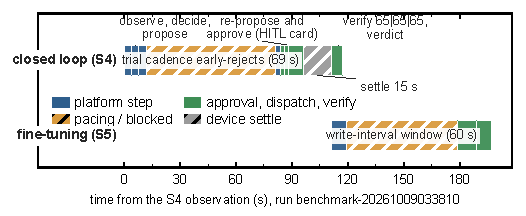
\includegraphics[width=\columnwidth]{resources/fig-process-campaign.pdf}
\caption{One governed iteration on the October 9 line: a corrective
decision ($0.276$\,g error) packaged by the proposer
as a sensitivity excitation; the trial cadence
early-rejects 69\,s before a human is involved; structured approval releases
the re-proposal, dispatch returns readback-verified, and the three-way check
reads 65|65|65. Lower lane: fine-tuning under the same 60\,s window,
rolled back and restored.}
\label{fig:loop}
\end{figure}

\subsection{Q1: Protocol Closure and Admission-Gate Attribution}
\label{sec:protocol}
\looseness=-1 On the five protocol lines the suite stores \resDaqSamples{} DAQ samples
through real drivers and dispatches governed writes over four protocol
families---about \resWriteNperLine{} writes each (\resPfiftyRange{} p50,
\resPninetyfiveRange{} p95; per-protocol values in the archived
metrics); the RTU-over-TCP
satellite is acquisition-only---readback confirmation where
supported---with one admission-record-verdict path per request. Each writable
line rejects 6/6 out-of-window probes (24/24) while accepting
its legal write. \looseness=-1 Two drills separate truth paths one success flag would collapse: a
frozen-measurement drill (write and readback consistent, measurement out of
window) ends with a system-judged backstop rollback \resBackstop{} later, and a
record-rollback drill restores the prior value by a separately admitted,
readback-confirmed write. A second preset with different signals and dynamics
is commissioned by configuration alone; across both presets 33 probes are
rejected on seven writable lines (24+9)---the same admission code
discriminating on unseen signal maps. The parameter
layer makes the interval geometry of Eq.~(\ref{eq:admission}) observable
(Fig.~\ref{fig:hitl}a): four declared layers narrow to one admitted
interval, each rejection attributable to its excluding layer;
a manual binding suspends a request visibly and unblocks it on approval
(latency \resHitlLatency, harness-adjudicated).

\looseness=-1 The ablation replays the same probes on companion run \resAblationRun{}
and a standalone fixture (six probe classes per arm, three deterministic
repetitions). Table~\ref{tab:ablation} reports
the four arms: full governance and the no-readback arm reject 18/18;
without the window interlock (alone or with the readback check) only
\resNoInterlockIntercept{} reject and the six window-class probes execute
and are journaled---prevention is the interlock's job; a relaxed
configuration degrades from prevention to detection, the readback check
retained to surface written-but-unconfirmed commands. The hard range is
structurally unbypassable---all four governed routes re-admit it at one
journaling entry point, per request (Section~\ref{sec:nodeexec})---and the
soft window is its removable part.

\begin{table}[!t]
\centering
\caption{Admission ablation on companion run \resAblationRun{}: six probe
classes per arm, three deterministic repetitions. The four hard-range
classes are rejected in every arm; only the two window-edge classes flip.}
\label{tab:ablation}
\scriptsize
\setlength{\tabcolsep}{2.2pt}
\renewcommand{\arraystretch}{0.95}
\begin{tabular}{@{}lcccc@{}}
\toprule
Arm & Soft win. & Readback & Intercept & Executed \\
\midrule
full & \checkmark & \checkmark & 18/18 & 0 \\
no-readback & \checkmark & --- & 18/18 & 0 \\
no-interlock & --- & \checkmark & 12/18 & 6 jour. \\
ungated & --- & --- & 12/18 & 6 jour. \\
\bottomrule
\end{tabular}
\end{table}

\subsection{Q2: The Agent-Team Optimization Workflow and Its Results}
\label{sec:agentteam}
\looseness=-1 The workflow ran end to end on the cast-film line and then a larger BOPET line
(Section~\ref{sec:reuse}); a scripted policy issued the writes (two live
engine turns follow). On the single-node
mission one write sufficed (\resMissionFrom\,$\rightarrow\,$\resMissionTo\,$^{\circ}$C
against target \resMissionTarget\,$^{\circ}$C,
settled at \resMissionPv\,$^{\circ}$C, journal-attributed, task
\texttt{COMPLETED}).
The BOPET mission is the multi-node case: nine devices and 49 signals
(\resBiaxSp{} writable, \resBiaxDaq{} readable), all ensure-pass created.
Three
governed writes on three distinct nodes---casting speed
$32\!\rightarrow\!33.8$\,m/min, fast-roll speed
$118\!\rightarrow\!120.3$\,m/min, and rail width $3000\!\rightarrow\!3035$\,mm---
bring thickness from \resBiaxStart{} to
\resBiaxFinal\,$\mu$m against
$\resBiaxTarget\pm\resBiaxTol$\,$\mu$m---$0.04$\,$\mu$m inside the window;
the same run's prose summary records it \emph{not} attained while its
machine-readable verdict records attained, so we report both; the verdict
matches the archived predicate, whose terminal observation sits inside the
window on re-check---the prose narration erred. Each write opened a record,
received \texttt{keep}, and left an
agent-attributed journal entry; the parent task reaching \texttt{COMPLETED}.
Finally,
two live agent-engine turns (omp adapter, glm-5.3-flash)
drove the same slot on a scratch line---a bounded write
(\resLlmWall), a goal-driven descent settling at
\resGoalFinal\,$\mu$m against a harness-supplied target ($52.0\pm0.8$\,$\mu$m,
in the task text, not the scenario predicate), and a recipe save
with attributed authorship (\resGoalWall). They show an engine
occupying the slot, not agent quality---the run's pass criterion is a
completion marker in the transcript.

\subsection{Q3: The Deterministic Closed Loop}
\label{sec:controller}
\looseness=-1 Seeds 42--44 each issue two governed writes with no rejection, raising the
cast-film objective $J$ from $J_{0}\approx\resJzero$ toward its grid
optimum ($J/J^{*}=\resControllerMin$--\resControllerMax{} against
$J^{*}=\resJstar$; the grid enumerates the admissible zone-temperature,
screw-speed, and line-speed setpoints, so $J^{*}$ lower-bounds the true
optimum and the reported ratio upper-bounds $J/J_{\text{true}}$). What the
benchmark establishes is narrower: the governed path
passes a conventional controller's writes through unmodified---admissible,
journaled, read back; the claim is transparency of evidence handling,
not a performance delta.

\subsection{Q4: Four Process Missions}
\label{sec:scenarios}
\looseness=-1 The campaign runs four blueprint-provisioned lines concurrently; in this run
(seed 42) all four attain their archived predicates---evaluated from
subsequent observations, not task state. Fig.~\ref{fig:missions} archives
each mission's optimization trajectory.
Injection molding is the minimal case (two writes: hold pressure
45$\rightarrow$58.2\,bar, hold time 6$\rightarrow$10.64\,s), BOPET the multi-node case of
Section~\ref{sec:agentteam}; both close with task state and predicate agreeing. \looseness=-1 Wastewater treatment (anaerobic--anoxic--oxic) is the write-heaviest
mission (\resWwtpWrites{} governed writes across distinct nodes---the
Section~\ref{sec:nodeexec} spacing is per node): dissolved oxygen rises from
\resWwtpStart{} into $3.4\pm0.6$\,mg/L (attainment window; terminal
observation 3.50\,mg/L, Fig.~\ref{fig:missions}b) under five
effluent guards: four guard margins finish wider than at baseline, and the
fifth, pH, drifts 6.59$\rightarrow$6.38. Its
most informative events are blower steps that were admissible and journaled
yet lost compliance margin; the verdict stage
reverted them---a bad proposal is rejected in the evidence, not at the
admission gate. Annealing starts far outside the hardness window
(\resAnnealStart\,HV at 140\,m/min); zone-3 temperature, one
zone-2 trim, and two
line-speed steps hold $95\pm6$\,HV while raising line speed by
\resAnnealGain, and a further attempt at \resAnnealSpeedTried\,m/min is
reverted for leaving the margin---on record. Mission clocks (\resInjWall,
\resWwtpWall, \resAnnealWall; BOPET's unarchived) are simulated mission
durations under accelerated dynamics; across the four missions in this
run, platform-side behavior is identical while the write economy---governed
writes per scripted policy---varies by more than a factor of seven
(2, 15, 5, and 3).

\begin{figure}[!t]
\centering
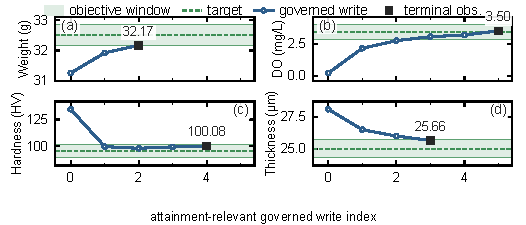
\includegraphics[width=\columnwidth]{resources/fig-missions.pdf}
\caption{Archived optimization trajectories of the four concurrent missions
(seed 42): observed controlled quantity after each
attainment-relevant governed write, against the archived objective window;
the index counts those writes ((b) plots 6 of its 15). (a) Injection
molding; (b) wastewater treatment (A2O); (c) annealing; (d) BOPET film.
Dissolved oxygen; observations under scripted policies.}
\label{fig:missions}
\end{figure}

\subsection{Q5: Deployment-Scale Regression and Write-Evidence Campaign}
\label{sec:hardening}
The final lens stresses the platform: the hardening pass made the
evidence grading, the master switch, and the approval-anchored dispatch
interval of Section~\ref{sec:mech} the explicit test surface of the
closed-loop, fine-tuning, and write-evidence scenarios.
\looseness=-1 \emph{Full-suite repeatability.} Nine pipeline executions
complete with zero failed checks (Table~\ref{tab:campaign}); October~7--8
runs wait out the remaining \resCadenceWait{} inside the
per-line trial cadence---pacing stays in force under automation.

\begin{table}[!t]
\centering
\caption{Campaign progression across the October passes; every execution
completes with zero failures.}
\label{tab:campaign}
\scriptsize
\setlength{\tabcolsep}{3.2pt}
\renewcommand{\arraystretch}{1.0}
\begin{tabular}{@{}llrl@{}}
\toprule
Executions & Test surface & Per run & Total \\
\midrule
October 7 (3 runs) & baseline S0--S7 suite & 79 & 237 \\
October 8 (3 runs) & + grading, master-switch checks & 90--92 & 273 \\
October 9 (3 runs) & same surface under live load & 90--92 & 272 \\
\midrule
nine executions & zero failed checks & --- & 782 \\
\bottomrule
\end{tabular}
\end{table}

\looseness=-1 \emph{Closed-loop scenario under governance.} Each run walks observation, decision (dead-band
\resNovDeadband, slope \resNovSlope), a five-element proposal,
HITL approval, batch dispatch, and three-way consistency (recipe, PLC
readback, mirror). The loop runs in two
regimes: October 7--8 descends $66\!\rightarrow\!63$\,bar one governed
step per run; October 9 answers a downward drift in the mirrored weight
(\resNovWeights) with a bounded zigzag
(\resNovZigzagFrom$\!\rightarrow\!$\resNovZigzagTo\,bar) and two
corrective steps (\resNovCorrFrom$\!\rightarrow\!$\resNovCorrTo\,bar)
answering residual error ($0.169/0.276$\,g)---the zigzag is deliberate
excitation, not a correction. Every step
verifies
equal values across the three sources at maximum consistency error
\resConsistencyErr{} ($0.05$\,bar device, $0.51$\,bar bucketed-mirror
tolerances---all legs equal at the endpoint's recording resolution). The pacing window acts before
the human: in two October~9 runs the proposal is early-rejected by the
trial cadence
and re-proposed \resNovCadenceReject{} later; only then is the HITL card
raised and structured approval releases the readback-verified dispatch
(Fig.~\ref{fig:loop}). Approval-to-dispatch takes \resHitlDispatchMs;
observation-to-verification spans \resObsVerifyFast{} without a pending
cadence window and 96.1\,s on October~9, \resObsVerifyCadence{} with one
(October~7)---the loop's time is governance, not platform overhead. The fine-tuning
scenario rides the same windows (Fig.~\ref{fig:loop}, lower lane);
the diagnostics scenario exports a 30-min merged wide
table (\resRowsRange{} rows)---a data-quality observation, not
a process excursion.

\looseness=-1 Latency and mission figures are single-run point estimates
(about \resWriteNperLine{} writes per line, one trajectory each); the Q1
approval latency is the harness's mediation span, not a human-response
measurement, and Q5's approval-to-dispatch span is server-side only. Only Q3
repeats across seeds, Q5's repetition is across consecutive deployment-tier
campaigns, and the Q1 ablation repeats deterministically
(Table~\ref{tab:ablation}); the campaign re-exercises the governance
surfaces (S1, S3) nine times with zero failures but does not re-run the
Q1--Q4 missions, which remain single-trace case studies, as are the
fault-suite grade outcomes (n=1--2 injected cases).

\looseness=-1 \emph{Write-evidence legs.} A dedicated seven-leg suite verifies Sections~\ref{sec:ack}
and~\ref{sec:hitl} directly in legs~(1)--(5): (1)~the master switch refuses an unconfirmed manual-to-automatic
transition; (2)~a mock-acknowledged (transport-acknowledged) dispatch is
promoted to readback-verified by post-write re-read;
(3)~a broker cut marks the affected parameter \emph{failed} at the batch
summary (operations level error) while its healthy sibling verifies;
(4)~a publish-only endpoint accepts the write (broker puback,
\texttt{ok=true}) yet stays \emph{unverified} through three verification
attempts---the receipt the Section~\ref{sec:ack} rule is stated
against; (5)~on a manual-mode line an approval-free binding's dispatch is
intercepted into the queue, approval releasing all six parameters
device-verified; (6)--(7)~API regression and documentation-consistency
suites close the campaign.

\looseness=-1 \emph{Observed grade distribution.} In fault-free operation,
every batch dispatch of the six hardened runs (October~8--9) closed
\emph{readback-verified}---structured approval released it and the three-way
check read equal values at \resConsistencyErr{} maximum error
(Fig.~\ref{fig:loop}). The non-verified grades appear only under the fault
suite's injected conditions, the distribution a healthy platform
should produce: \resAckFailed{} \emph{failed} (broker unreachable; healthy
sibling verified), \resAckUnverified{} \emph{unverified} (publish-only
endpoint, three attempts), and \resAckPromoted{} parameters promoted from
transport-acknowledged receipts to readback-verified by post-write re-read.
The remaining terminal grade, transport-acknowledged, occurs on MES-style
endpoints that return an application-level acceptance without a readback
mapping; the platform's MES route tests cover it, but the campaign archives
MES in read mode only---a disclosed gap in the campaign's
write-evidence coverage.

\looseness=-1 Across the five questions, the mechanisms of
Section~\ref{sec:mech} behave as specified.


\section{Discussion and Limitations}
\label{sec:limits}
\subsection{Validity and Reproducibility}
\looseness=-1 Run identifier, seed, commit, harness fingerprint, and raw artifacts are
fixed, so counts are re-derivable rather than trusted; Q5 adds per-run
ledgers and timelines. Five
qualifications bound what they support: simulation-tier evidence
(deterministic per seed; no physical-device
campaign, operator study, or external comparison reported); internal-oracle
optima and predicates under an author-implemented, author-adjudicated
harness and simulator set; single-host latencies and near-contemporary runs;
implemented-but-unexercised capabilities and a
single live provider/model;
and harness-adjudicated approval (human decision latency and quality out of
scope).
\subsection{Safety Positioning and Human Oversight}
\looseness=-1 The threat model is a misbehaving or manipulated agent inside
an otherwise trusted platform and plant; approval dialog, admission
re-checks, and journaling are the containment surfaces; no injection
campaign or approval-dialog operator study is reported; stolen credentials
and compromised endpoints are the domain of IEC~62443
\cite{iec62443-3-3}, and high-risk-AI regulatory
duties---record keeping and human oversight---belong to instruments such
as Regulation (EU) 2024/1689 \cite{eu2024aiact}; the
attributed journal and approval gates serve its logging and
oversight articles at the evidence layer, certification out of scope.
Fast regulation, hardware interlocks,
and safety functions remain in the PLC; prompts and retrieved documents are
untrusted text, not authority
\cite{greshake2023injection,liu2024pinjection}---the proposer is confined to
per-binding scope and journaled, attributable actions: a bounded blast
radius, not a protection guarantee.
Admission limits,
acknowledgment grading, and the backstop run with or without human
approval---enforcement never queues behind human attention (the
deferred-mode exception hands actuation back to the approval policy,
Section~\ref{sec:agentloop}). The pacing
windows bound approval demand per line, and
batch release (Section~\ref{sec:hardening}, leg~5) is the demonstrated
fatigue mitigation; approval fatigue and automation bias remain
human-factors risks
\cite{parasuramanmanzey2010complacency,bainbridge1983ironies}. A lead agent's
delegation-mode choice (Section~\ref{sec:hitl}) is the one agent-reachable
path around per-request approval; capping the granted mode at the granter's
own binding mode, or requiring the line-switch confirmation for it, is
queued as the guard, alongside the verdict-side guard of
Section~\ref{sec:agentloop} (an independent adjudication identity, or a
platform-side minimum re-check before \texttt{keep}).

\subsection{Deployment Boundaries}
\looseness=-1 Against the nearest systems of Section~\ref{sec:related},
the differentiator is not the LLM---a replaceable strategy slot---but the
production-scoped authority and evidence around its writes: no nearest
system reports that combination on one path. The layer installs beside the
plant's protocol endpoints, onboards declaratively
(Section~\ref{sec:reuse}), and leaves PLC protection and DCS interlocks
untouched.
Execution and recovery are non-atomic: bookkeeping may fail after actuation, the
pacing windows time writes rather than certify
stability, declared per-write step limits are advisory metadata surfaced to
agents rather than enforced bounds, and multi-node compensation may partially
succeed. Readback agreement and three-way
consistency need not imply process recovery; hold heartbeats re-apply the
stored setpoint without re-admission, trailing a narrowed window.
Oscillation, storage failure, clock error, concurrency beyond the four-line
campaign, and split-brain supervisor deployments with divergent stores
remain unevaluated; the journal is append-only but not
tamper-evident---no hash chain or trusted timestamping---so forensic
integrity rests on host security, and clock skew propagates into timeline
evidence. A supervisor outage halts dispatch rather than permitting writes
through; plant staff retain their conventional
DCS/SCADA stations outside \system{}---the governed path mediates
agent-originated and platform-client writes, not existing operator
tooling: an integration boundary, not a takeover. The next
evidence tiers are a
hardware-in-the-loop leg against a
real PLC or OPC-UA endpoint and community benchmarks such as Tennessee
Eastman \cite{downs1993tep} or Secure Water Treatment \cite{goh2017swat}. Production
integration additionally requires change-controlled bound changes with
process-evidence validation, approval/open-record aging and
backstop-deferred states surfaced on the plant alarm system, the
bench-mode switch refused at production boot, and
approval as workflow mediation---attribution and timestamp, not an
electronic signature. \looseness=-1 In production, bindings govern
sanctioned tools, not arbitrary privileged-engine I/O---least privilege,
endpoint security, and IT/OT separation remain necessary
\cite{iec62443-3-3}; \system{} is neither a safety
instrumented function nor a plant-protection substitute \cite{iec61511};
line-scoped approver authorization is still missing, so production needs
segregation of duties and alarm-path failure tests \cite{isa182}.

\section{Conclusion}
\label{sec:conclusion}
\looseness=-1 \system{} contributes a governed supervisory execution layer rather
than a new process optimizer: one governed path from agent-team identities
through semantic nodes and production context to governed writes, graded
acknowledgments, verdicts, and compensation---admission, approval, and
recovery left as separately inspectable, actor-attributed evidence on every
agent-originated write. Physical-plant
deployment, operator studies, and
external-framework comparison remain open; until then, optimization
benefit, autonomous control, and safety assurance stay unsupported claims.

\vspace{2pt}\noindent\textit{Data availability and disclosure.}
Artifacts are archived per run in the project's benchmark result tree; the
platform and its deterministic simulators are publicly available
(Section~\ref{sec:arch}). The live engine-turn transcripts
(Section~\ref{sec:agentteam}) were excluded by the log-retention rule and
survive only as recorded outcomes; the
write-evidence suite is rerunnable from its script. AI assistants supported
editing under author direction; the authors remain responsible for all
claims.


\bibliographystyle{IEEEtran}
% Keep IEEEtran's default bibliography size and leading.
\bibliography{resources/refs}

\end{document}
